\documentclass[11pt]{article}

\usepackage[margin=1in]{geometry}
\usepackage[T1]{fontenc}
\usepackage[utf8]{inputenc}
\usepackage{lmodern}
\usepackage{microtype}
\usepackage{amsmath}
\usepackage{graphicx}
\usepackage{float}
\usepackage{booktabs}
\usepackage{array}
\usepackage{caption}
\usepackage{subcaption}
\usepackage{hyperref}
\hypersetup{colorlinks=true,linkcolor=blue,urlcolor=blue}

\title{Entrega 2 --- Predicción de Churn en E-commerce (Olist)\\
\large Modelos, MLflow en EC2 y Tablero}
\author{
David Alan Delgado Zarco \\
Octavio Esquivel Alvarez del Castillo \\
John Williams Morrill \\
Jason Rosher Morrill
}
\date{\today}

\begin{document}
\maketitle

\begin{abstract}
Este documento presenta la implementación de un modelo de predicción de churn (abandono) para clientes del dataset Olist, siguiendo la definición operacional de la Entrega 1 con ventana $W=90$ días. Para evitar \textit{leakage} temporal, el label se define observando compras en una ventana futura posterior a una fecha de \textit{snapshot}. Se construyen features a nivel \texttt{customer\_unique\_id} (RFM y experiencia), se aplica una partición temporal train/test y se comparan modelos (Regresión Logística vs. Random Forest), evaluando especialmente la clase minoritaria (no-churn/recompra). Los experimentos se registran y comparan en MLflow desplegado en AWS EC2, y se construye un tablero funcional (Streamlit) que muestra predicciones, umbral operativo y visualizaciones macro.
\end{abstract}

\section{Cambios vs. Entrega 1}
\begin{itemize}
  \item Se corrigió la definición del target: se eliminó el criterio trivial \texttt{churned = Recency > W} y se implementó un esquema \textit{snapshot + ventana futura} $(t, t+W]$.
  \item Se evitó \textit{leakage} temporal: features calculadas solo con historial previo al snapshot y partición temporal (no aleatoria).
  \item Se ajustó la población objetivo usando un \textit{lookback} para enfocarse en clientes activos (evita incluir clientes históricamente inactivos).
  \item Se amplió el soporte experimental: ejecución y comparación de runs en MLflow en una instancia AWS EC2 (con evidencias de IP/usuario).
  \item Se implementó un tablero funcional que consume el modelo ganador y muestra predicción, umbral y vistas macro.
\end{itemize}

\section{Datos y construcción del label}
\subsection*{Fuentes de datos}
Se utilizaron los archivos del dataset Olist: \texttt{orders}, \texttt{customers}, \texttt{payments}, \texttt{reviews} e \texttt{items}. Para evitar duplicación por relaciones 1:N, se agregaron pagos, reviews e items por \texttt{order\_id} antes de construir el dataset a nivel cliente.

\subsection*{Construcción del label (churn)}
Se definió una fecha de \textit{snapshot} y una ventana futura $W=90$ días. El churn se define como:
\[
churn=1 \Leftrightarrow \text{el cliente no realiza compras en } (snapshot, snapshot+W]
\]
y $churn=0$ en caso contrario (recompra). Para evitar sesgos por clientes históricamente inactivos, se filtra la población a clientes con compra reciente dentro de un \textit{lookback} previo al snapshot.

\subsection*{Evidencia de integridad del dataset}
En el preprocesamiento a nivel orden se verificó que no hubiera duplicación de \texttt{order\_id} (duplicados = 0), evitando inflación artificial de montos o conteos.

\section{Features y partición temporal}
\subsection*{Features}
Se construyeron features a nivel \texttt{customer\_unique\_id}:
\begin{itemize}
  \item \textbf{RFM}: Recency, Frequency, Monetary.
  \item \textbf{Experiencia/logística}: promedio de review score, días de entrega, retraso vs. fecha estimada, número de items, suma de precio y flete.
  \item \textbf{Contexto}: estado del cliente (\texttt{customer\_state}).
\end{itemize}

\subsection*{Partición temporal}
Se realizó un split temporal basado en la última compra del cliente (previa al snapshot), con un percentil (p.ej. 80\%) para separar train/test. Esto evita \textit{leakage} y refleja un escenario realista de generalización temporal.

\section{Modelos y evaluación}
\subsection*{Baseline por desbalance}
El dataset presenta alto desbalance (baja recompra). Por ello, se reportó un baseline trivial que predice churn para todos: logra accuracy alta pero F1 para no-churn es 0. Esto justifica el uso de métricas enfocadas a la clase minoritaria.

\subsection*{Modelos}
Se compararon:
\begin{itemize}
  \item \textbf{Regresión logística} (con \texttt{class\_weight=balanced}), variando $C$ y el umbral de decisión.
  \item \textbf{Random Forest} (con \texttt{class\_weight=balanced\_subsample}), con variantes de \texttt{max\_depth} y \texttt{min\_samples\_leaf}.
\end{itemize}

\subsection*{Métricas}
Además de accuracy, se reportaron métricas relevantes para no-churn (recompra): \texttt{pr\_auc\_nochurn\_0} y \texttt{f1\_nochurn\_0}, junto con matrices de confusión y curvas Precision--Recall para la clase no-churn.

\subsection*{Selección de umbral}
Se optimizó el umbral para maximizar \texttt{f1\_nochurn\_0}. En los experimentos se obtuvo un umbral operativo de 0.12.

\noindent \textbf{Run ganador (MLflow).} Se seleccionó el run \texttt{logreg\_C0.1\_thr012} por obtener el mejor valor de \texttt{pr\_auc\_nochurn\_0} (y un alto \texttt{f1\_nochurn\_0}) en la comparación de runs.



\begin{figure}[H]
\centering
\begin{subfigure}[b]{0.48\textwidth}
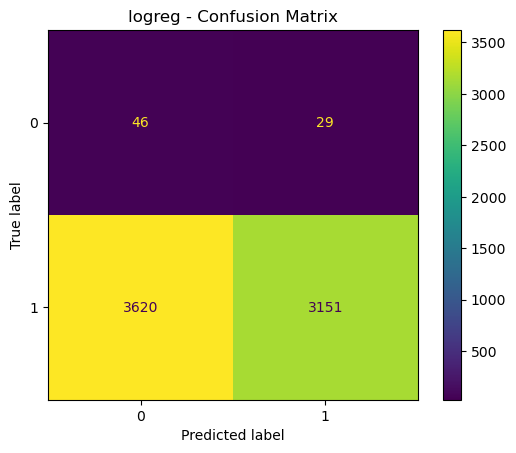
\includegraphics[width=\textwidth]{evidence/model/FIG_MODEL_01_cm_logreg.png}
\caption{Matriz de confusión (LogReg).}
\end{subfigure}\hfill
\begin{subfigure}[b]{0.48\textwidth}
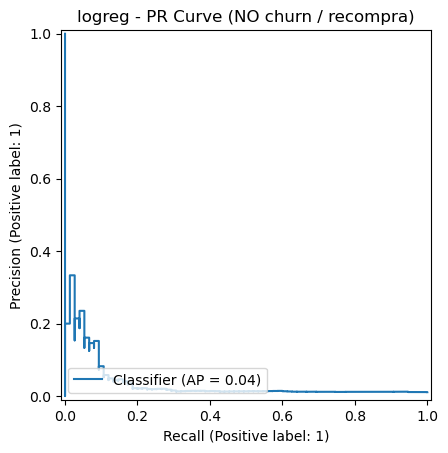
\includegraphics[width=\textwidth]{evidence/model/FIG_MODEL_02_pr_logreg.png}
\caption{Curva PR para no-churn (LogReg).}
\end{subfigure}
\caption{Evaluación del modelo.}
\end{figure}

\section{Soportes en MLflow (AWS EC2)}
\subsection*{Despliegue de MLflow en EC2}
Se desplegó MLflow Tracking Server en AWS EC2 (puerto 5000) con backend store SQLite y almacenamiento de artefactos en \texttt{/home/ubuntu/mlruns}. Se documentan evidencias con IP pública y usuario.

\begin{figure}[H]
\centering
\includegraphics[width=0.75\textwidth]{evidence/aws/EVID_AWS_01_ec2_whoami_ip.png}
\caption{Evidencia de ejecución en EC2 (usuario e IP).}
\end{figure}

\begin{figure}[p]
\vspace*{\fill}
\centering

\begin{subfigure}{0.85\textwidth}
  \centering
  \includegraphics[width=\textwidth]{evidence/mlflow/EVID_MLFLOW_01_ui_ip.png}
  \caption{UI MLflow con IP pública.}
\end{subfigure}

\vspace{1em}

\begin{subfigure}{0.85\textwidth}
  \centering
  \includegraphics[width=\textwidth]{evidence/mlflow/EVID_MLFLOW_02_runs_list.png}
  \caption{Lista de runs del experimento.}
\end{subfigure}

\caption{Acceso a MLflow y evidencia de experimentos.}
\vspace*{\fill}
\end{figure}

\subsection*{Comparación de runs}
\begin{figure}[H]
\centering
\includegraphics[width=0.85\textwidth]{evidence/mlflow/EVID_MLFLOW_03_compare.png}
\caption{Comparación de runs en MLflow (Compare). Recomendación: mostrar \texttt{pr\_auc\_nochurn\_0} y \texttt{f1\_nochurn\_0}.}
\end{figure}

\subsection*{Run ganador}
\begin{figure}[H]
\centering
\includegraphics[width=0.85\textwidth]{evidence/mlflow/EVID_MLFLOW_04_best_run_detail_params_metrics.png}
\caption{Detalle del run ganador: params y metrics.}
\end{figure}

\begin{figure}[H]
\centering
\includegraphics[width=0.85\textwidth]{evidence/mlflow/EVID_MLFLOW_04_best_run_detail_artifacts.png}
\caption{Detalle del run ganador: artifacts.}
\end{figure}


\section{Tablero}
\subsection*{Descripción}
Se desarrolló un tablero funcional (Streamlit) que permite:
\begin{itemize}
  \item Seleccionar cliente (\texttt{customer\_unique\_id}) y filtrar por estado.
  \item Visualizar $p(churn)$, umbral operativo y nivel de riesgo.
  \item Consultar features del cliente y exportar el resultado en JSON.
  \item Revisar visualizaciones macro: distribución de churn y tasa de churn por estado.
\end{itemize}

\begin{figure}[H]
\centering
\begin{subfigure}[b]{0.42\textwidth}

\includegraphics[width=\textwidth]{evidence/dashboard/EVID_DASH_01_prediction.png}
\caption{Tablero: predicción individual con umbral.}
\end{subfigure}\hfill
\begin{subfigure}[b]{0.4588\textwidth}

\includegraphics[width=\textwidth]{evidence/dashboard/EVID_DASH_03_features_export.png}
\caption{Tablero: features del cliente y export.}
\end{subfigure}
\caption{Tablero: features del cliente y export.}
\end{figure}

\begin{figure}[H]
\centering

\includegraphics[width=0.55\textwidth]{evidence/dashboard/EVID_DASH_02_macro.png}
\caption{Tablero: visualizaciones macro.}
\end{figure}

\section{Conclusiones y trabajo futuro}
\begin{itemize}
  \item El dataset presenta fuerte desbalance; accuracy no es suficiente. El baseline que predice churn para todos logra alta accuracy pero no identifica recompra (no-churn).
  \item La Regresión Logística supera a Random Forest en métricas de no-churn (PR-AUC/F1), por lo que se selecciona como modelo final.
  \item Se optimizó el umbral de decisión y se definió un umbral operativo de 0.12 para mejorar la detección de no-churn.
  \item MLflow en EC2 permitió comparar runs y conservar artefactos (matrices, curvas PR y modelos).
  \item Trabajo futuro: incorporar features por categoría/producto, calibración de probabilidades y evaluación basada en costos.
  \item La Regresión Logística superó a Random Forest en métricas de no-churn (PR-AUC/F1). El run \texttt{logreg\_C0.1\_thr012} se seleccionó como ganador en MLflow por su mejor \texttt{pr\_auc\_nochurn\_0}.
\end{itemize}

\end{document}